\documentclass{beamer}
\usepackage{mathrsfs} %Pretty fonts
\usepackage{amsmath}
\usepackage{amssymb}
\usepackage{amsfonts}
\usepackage{amsthm}
\usepackage{bbm}
\usepackage{tikz}
\usetikzlibrary{arrows,shapes,positioning}

\newtheorem{proposition}{Proposition}[section]

\mode<presentation>{\usetheme{Madrid}}
%%%% COMMANDS %%%%
% Real Numbers
\newcommand{\RNums}{\mathbb{R}}
% sigma-algebra
\newcommand{\salg}{\sigma\text{-algebra}}
% borel sigma-algebra
\newcommand{\borelsalg}{\mathscr{B}(\RNums)}
% Indicator function
\newcommand{\ind}{\mathbbm{1}}
% F: Sigma Algebra
\newcommand{\salgF}{\mathscr{F}}
% Probability P (P measure)
\newcommand{\Pm}{\mathbb{P}}
% Expectation's E
\newcommand{\E}{\mathbb{E}}
% Variance
\newcommand{\V}{\mathbb{V}}
% Continuous time stochastic process
\newcommand{\ctspr}{\{X_t\}_{t\geq 0}}
% Discrete time stochastic process
\newcommand{\dtspr}{\{X_n\}_{n\geq 0}}
% Insert only one number in the "align" environment
\newcommand\numberthis{\addtocounter{equation}{1}\tag{\theequation}}
% Measure Space
\newcommand{\MeasureSpace}[1]{(\Omega, \salgF, #1)}
% Proabability Space
\newcommand{\ProbSpace}{\MeasureSpace{\Pm}}
% Norm
\newcommand{\norm}[1]{\left\lVert#1\right\rVert}
% Inner Product
\newcommand{\innerprod}[2]{\langle #1, #2\rangle}


\title{Theoretical Grounds and Market Adaptations of Financial Fx and Interest Rate Options}
\author{Gerardo Dur\'an Mart\'in}
\institute{Universidad Marista}

\logo{\includegraphics[height=1.7cm]{UMA_logo}}

\begin{document}
%Generates the title page
\frame{\titlepage}

\AtBeginSection[]{
\begin{frame}
	\frametitle{Table of Contents}
	\tableofcontents[currentsection]
\end{frame}
}

\section{Financial Markets}

%% Market Assumptions
\begin{frame}
\frametitle{Some Important Definitions}

\only<1->{
\begin{definition}[Security]
	A security is an instrument that either represents ownership or that derives its value from a commodity.
\end{definition}
}

\only<2->{
\begin{definition}[Market]
	A market is the place where buyers meet sellers to exchange securities.
\end{definition}
}

\only<3->{
\begin{definition}[Arbitrage]
	We define an arbitrage as the probability of making a risk-free profit from a suitable market strategy.
	$$
		\Pm{(\text{Risk-free profit} > 0)} = 1
	$$
\end{definition}
}
\end{frame}


\begin{frame}
\frametitle{Market Assumptions}
\begin{itemize}
	\item Many buyers and sellers (liquidity);
	\item possible to lend and borrow at the same rate interest rate $r$;
	\item Market participants take advantage of arbitrage opportunity, thereby correcting any deviation from the actual value of any asset.
	\item All participants have the same information.
\end{itemize}
\end{frame}

%% Instruments
\begin{frame}
\frametitle{The Instruments}
	
	\begin{columns}[c]	
	
	\column{0.45\textwidth}
	\begin{itemize}
		\item <1-| alert@1> Bonds
		\item <2-| alert@2> Stocks
		\item <3-| alert@3> Foreign Exchange Currencies
		\item <4-| alert@4> Derivatives
	\end{itemize}
	
	\column{0.5\textwidth}
	\only<1>{
	A Bond is a debt obligation, its main function is to raise capital for the issuer of the bond. In turn, the buyer of the bond receives interest on the amount loaned.
	}
	\only<2>{
	A stock is a security that represents ownership on a fraction of a corporation. The return on the company for the owner of a stock is represented as a dividend.
	}
	\only<3>{
	``One country’s currency freely convertible in the foreign exchange market.'' (Kozikowski, 2013)
	}
	\only<4>{
	``[A derivative is] a financial instrument whose value depends on (or derives from) the values of other, more basic, underlying variables.'' (Hull, 2014)
	}
	\end{columns}
\end{frame}

%%Forwards
\begin{frame}
\frametitle{Derivatives: An Example}

	\begin{definition}[Forward]
		A forward is a derivative contract that gives the buyer both the right, and the obligation to to purchase a specified amount of the stock at some future time $T$, at a price $K$. The value of the forward today is 0.
	\end{definition}
	The payoff of the forward is $S_T - K$. What is the $K$ such that the contract has zero value today and has no possibility of arbitrage?
	
	\begin{figure}
	\includegraphics[width=0.45\textwidth]{../images/foward_payoff}
	\end{figure}
\end{frame}

\begin{frame}
\frametitle{Derivatives: An Example (cont'd)}
Assume a continuously compounded interest rate $r$, denote $S_t$ the value of the stock at time $t$. At $t=T$ the value of the forward is
$$
	S_T - K = 0
$$

By no arbitrage, the present value of the strategy is
$$
	S_0 - Ke^{-rT} = 0 \implies K = S_0e^{rT}
$$
Therefore, $S_0e^{rT}$ is the the value that guarantees no arbitrage.
\end{frame}

\begin{frame}
\frametitle{Derivatives: An Example (cont'd)}

(Why?)

Assume $K^\prime > K = S_0e^{rT}$. 
\begin{itemize}
	\item At $t=0$, borrow $S_0$; purchase the stock; and take a short position the forward contract.
	\item At $t=T$, receive $K^\prime$; give the forward; and repay $S_0e^{rT}$. Profit $K^\prime - S_0e^{rT}$.
\end{itemize}

The same can be said for $K^\prime < K$, by taking a long position.
\end{frame}

%%Option Pricing
\begin{frame}
\frametitle{Derivatives: Another Example}

\begin{definition}[European Call Option]
A European call option is a derivative contract that gives the buyer the right, but not the obligation to purchase a specified amount of stock at some future time $T$, at a price $K$.
\end{definition}

The payoff of the option is $\max\{S_T - K, 0\}$. What is the price of the option today that guarantees no arbitrage?

\begin{figure}
	\includegraphics[width=0.45\textwidth=]{../images/Call}
\end{figure}
\end{frame}

\section{Probability and Measure Theory}
\begin{frame}
\frametitle{Probability Theory}

We will work on the following probability space.
\begin{definition}[Probability Space: Kolmogorov's Axiom System]
An ordered tripe $\ProbSpace$ where
\begin{itemize}
	\item $\Omega$ is a set of points $\omega$;
	\item $\salgF$ is a $\salg$ of elements of $\Omega$; and
	\item $\Pm$ is a probability on $\salgF$. 
\end{itemize}
\end{definition}

\begin{definition}[Random Variable]
	\[
		X^{-1}(B) = \{\omega \in \Omega | X(\omega) \in B\} \ \forall \ B \subseteq \borelsalg.
	\]
\end{definition}
\end{frame}

%% Integrals
\begin{frame}
\frametitle{Integrals}

\only<1>{
\begin{definition}[Integral v.1]
	Let $\MeasureSpace{\mu}$ be a measure space, we define the Lebesgue integral (or integral)of the indicator function $\ind_A$ w.r.t. $\mu$ as
	\[
		\int_\Omega \ind_A d\mu := \mu(A)
	\]
\end{definition}
}

\only<2>{
\begin{definition}[Simple Function]
	Let $(\Omega, \salgF)$ a measurable space and $X$ an $\salgF$-measurable function. It is said that $X$ is a \textbf{simple function} if it takes only a unique finite number of values $\{x_i\}_{i=1}^{n} \in \RNums$ over measurable sets $\{A_i\}$. Then, $X$ can be written as
	\[
		X(\omega) = \sum_{i=1}^{n}x_i\ind_{A_i}
	\]
\end{definition}

\begin{definition}[Integral v.2]
	let $X$ be a simple function, we define the integral of $X$ w.r.t. $\mu$ as:
	\[
		\int_\Omega X(\omega) d\mu(\omega) := \sum_{i=1}^{n}x_i\mu(A_i)
	\]
\end{definition}
}

\only<3>{
\begin{definition}[Integral v.3]
For any nonnegative function $X$, we define the integral of $X$ w.r.t. a measure $\mu$ as
\[
	\int_\Omega Xd\mu := \sup\left\{\int_\Omega h d\mu \ | \ 0 \leq h \leq X \text{, $h$ is simple}\right\}
\]
\end{definition}
\begin{figure}
	\includegraphics[width=0.50\textwidth]{../images/simple_sine}
\end{figure}
}
\end{frame}

\begin{frame}
If $X$ is any measurable function, we define the positive and negative parts of $X$ as:
\begin{align}
	X^+ := \max\{X(\omega), 0\} \\
	X^- := \max\{-X(\omega), 0\}
\end{align}

Thus, $X = X^+ - X^-$, and $|X| = X^+ + X^-$. Since both parts of $X$ are positive, their integrals are well defined.\\

\begin{definition}[$L_1$ spaces]
We denote by $L_1 \equiv L_1\MeasureSpace{\mu}$ the family of integrable functions w.r.t. $\mu$. Note that $X \in L_1$ if and only if $|X| \in L_1$. i.e.,

\begin{equation}
	\int_\Omega |X| d\mu = \int_\Omega X^+ d\mu + \int_\Omega X^- d\mu < \infty
\end{equation}
\end{definition}
\end{frame}

\begin{frame}
\begin{proposition}
	For any $X$, $Y$ $\salgF$-measurable functions in $L_1$; $A$, $B$ members of $\salgF$:
	\[
		X \geq 0 \implies \int_\Omega X d\mu \geq 0
	\]
	
	If $X \leq Y$ (monotonicity),
	\[
		\int_\Omega X d\mu \leq \int_\Omega Y d\mu
	\]
	
	If $A \subseteq B$ and $X \geq 0$,
	\[
		\int_A X d\mu \leq \int_B X d\mu
	\]
	
	If $\alpha$, $\beta$ $\in \RNums$ (linearity),
	\[
	\int_\Omega (\alpha X + \beta Y) d\mu = \alpha \int_\Omega X d\mu + \beta \int_\Omega Y d\mu
	\]
\end{proposition}
\end{frame}

\begin{frame}
\begin{theorem}[\textbf{Radon Nikodym Theorem}]\label{th:radon-nikodym}
Let $\mu$ and $\lambda$ be $\sigma$-finite positive measures defined on $(\Omega, \mathscr{F})$ such that, for every $A \in \mathscr{F}$, $\lambda(A) = 0 \implies \mu(A)= 0$. Then, there exists a function $f: \Omega \to [0, \infty]$ such that
\[
	\mu(A) = \int_A f d\lambda.
\]

Where the function $f$ is defined up to sets with measure zero. $f$ is sometimes called the Radon-Nikodym derivative and it can be written as $\frac{d\mu}{d\lambda}$
\end{theorem}

\end{frame}

%% Expectation
\begin{frame}
\frametitle{Expectation}
	\begin{definition}
		Let $X$ be a r.v. on $\ProbSpace$, we define the expectation of $X$ with respect to (w.r.t.) $\Pm$ as
		\[
			\E[X] := \int_\Omega X(\omega) d\Pm(\omega)
		\]
	\end{definition}
	
	\begin{definition}[Conditional Expectation w.r.t. a $\sigma$-algebra]
The conditional expectation of a nonnegative random variable $X$ with respect to the $\sigma$-algebra $\mathscr{G}$ is a nonnegative random variable denoted $\mathbb{E}[X | \mathscr{G}]$ or $\mathbb{E}[X | \mathscr{G}](\omega)$ such that,
\begin{enumerate}
	\item $\mathbb{E}[X | \mathscr{G}]$ is $\mathscr{G}$-measurable; and
	\item For every $A \in \mathscr{G}$,
	\[\int_A X d\Pm = \int_A \mathbb{E}[X | \mathscr{G}] d\Pm\].
\end{enumerate}
\end{definition}
\end{frame}

\begin{frame}
\begin{proposition}
	\begin{enumerate}
		\item If $a, b \in \RNums$, $\E[\alpha X + \beta Y | \mathscr{G}]$ = $\alpha \E[X | \mathscr{G}] + \beta\E[Y | \mathscr{G}]$;
		\item $\E[\E[X | \salgF]] = \E[X]$;
		\item $\E[\E[X | \salgF_2] | \salgF_1]$ = $[X | \salgF_1]$ if $\salgF_1 \subseteq \salgF_2$;
		\item $\E[\E[X | \salgF_2] | \salgF_1]$ = $[X | \salgF_2]$ if $\salgF_2 \subseteq \salgF_1$; and
		\item Let $X$ be a random variable such that $X \perp \mathscr{G}$ then, $\E[X|\mathscr{G}] = \E[X]$. Consequently, for any borel-measurable function $h$, $\E[h(X)|\mathscr{G}] = \E[h(X)]$.
	\end{enumerate}
\end{proposition}
\end{frame}

\begin{frame}
\frametitle{Stochastic Processes}

\only<1>{
\begin{definition}[\textbf{Stochastic Process}]
	Let $\ProbSpace$ be a probability space. A stochastic process is a set of random variables that takes values in some set $S$ called the \textbf{state space}, and are indexed by some set $T$.
	\begin{equation}
		\{X_t \ | \ t \in T\}.
	\end{equation}
\end{definition}
We can consider a stochastic process as a two variable function
\[
	X: T\times\Omega \to S
\]

Where,
\begin{enumerate}
	\item For for fixed $t\in T$, $\omega \to X_t(\omega)$ is random variable; and
	\item for fixed $\omega \in \Omega$, $t \to X_t(\omega)$ is the path of the process.
\end{enumerate}
}

\only<2>{
\begin{figure}
\centering
\includegraphics[width=0.9\textwidth]{../images/stoch_process_3d}
\caption{Distribution and Path of a Stochastic Process.}
\end{figure}
}
\end{frame}

\begin{frame}
\begin{definition}[\textbf{Martingale}]\label{def:martingale}
	An stochastic process $\ctspr$ defined over $\ProbSpace$ is said to be a martingale w.r.t. a filtration $\{\salgF_n\}_{n\geq 0}$ if, for all $t \geq 0$, and $t \leq s$,
	\begin{enumerate}
		\item $X_t$ is $\salgF_t$-measurable;
		\item $X_t$ is in $L_1$ (i.e. is is measurable for all $t$); and
		\item $\E[X_t | \salgF_s] = X_t$.
	\end{enumerate}
\end{definition}
\end{frame}


\section{Option Pricing: A primer}
\begin{frame}
\frametitle{One Step Binomial Model}
We assume a simple market consisting of a stock and a cash bond.
\begin{itemize}
	\item<1->{\textbf{The Stock}\\
	\begin{figure}[h!]
\centering
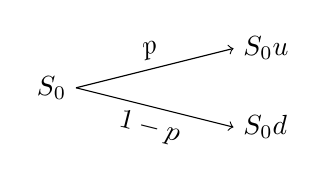
\begin{tikzpicture}
    \draw[->] (0,0) node[left]{$S_0$} --(2, 0.5) node[pos=0.5, sloped, above] {$p$};
    \node[right] at (2, 0.5) {$S_0u$};

    \draw[->] (0,0) --(2, -0.5) node[pos=0.5, sloped, below] {$1-p$};
    \node[right] at (2, -0.5) {$S_0d$};
\end{tikzpicture}
\end{figure}
Stock has value $S_0$ at outset. Between any two units of time, the stock can either go up by a factor $u$ (with probability $p$), or down by a factor $d$ (with probability $1-p$).
}
	\item<2>{\textbf{The Cash Bond}\\
	Represents the time value of money. $B_0$ invested at $t=0$ grows to $B_0e^{rT}$ one period thereafter.
	}
\end{itemize}
\end{frame}

\begin{frame}
	This simple market yields the possibility for a derivatives' market, i.e., there could be a payoff with price $f_0$ today that derives its value from the possible directions the stock may take: either $f_u$ if it goes up, or $f_d$ otherwise.
\begin{figure}
	
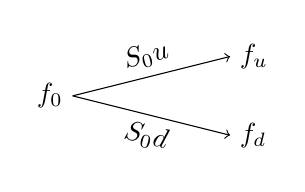
\begin{tikzpicture}
    \draw[->] (0,0) node[left]{$f_0$} --(2, 0.5) node[pos=0.5, sloped, above] {$S_0u$};
    \node[right] at (2, 0.5) {$f_u$};
    \draw[->] (0,0) --(2, -0.5) node[pos=0.5, sloped, below] {$S_0d$};
    \node[right] at (2, -0.5) {$f_d$};
\end{tikzpicture}
\end{figure}
\end{frame}

\begin{frame}
(Why?)
Consider the portfolio $(\phi, \psi)$ with $\phi$ number of stocks, and $\psi$ amount in the bank. The value of the portfolio at $t=0$ is
\[
    \phi S_0 + \psi B_0
\]
We derive a payoff $f$ contingent of the movement of the stock. At $t=\delta_t$ we have
\begin{align*}
    \phi S_0u + \psi B_0e^{r \delta_t} = f_u\\
    \phi S_0d + \psi B_0e^{r \delta_t} = f_d
\end{align*}

Yields,
\begin{align}
	\phi &= \frac{f_u - f_d}{S_0(u-d)}\\
	\psi &= e^{-r\delta_t} \frac{uf_d - df_u}{u -d}
\end{align}
\end{frame}

\begin{frame}
Therefore, buying the portfolio $(\phi, \psi)$ guarantees the payoff at $t=\delta_t$ (a risk-free strategy). Denote $\mathcal{V}$ the value of the portfolio at $t=0$.
\begin{equation} \label{eq:v_price_complete}
	\mathcal{V} = e^{-r\delta_t}\left[f_u \frac{e^{r\delta_t} - d}{u - d} + f_d \frac{u - e^{r\delta_t}}{u-d}\right].
\end{equation}

$\mathcal{V}$ is the cost of a risk-free strategy that guarantees the payoff. Furthermore, showing that $d < \exp{(r\delta_t)} < u$ proves that there exists no possibility of arbitrage.
\end{frame}

\begin{frame}
Denote
\begin{equation}
    q:= \frac{\exp{r\delta_t} - d}{u - d} \Longrightarrow 1-q = \frac{u - \exp{(r\delta_t)}}{u-d}.
\end{equation}

We rewrite (\ref{eq:v_price_complete}) as
\begin{equation} \label{eq:v_price}
    \mathcal{V} = \exp{(-r\delta_t)}[S_0u\cdot q + S_0d \cdot (1-q)] = \E_{\mathbb{Q}}[\mathcal{V}_{\delta_t}|\salgF_0].
\end{equation}
$\mathcal V$ is the discounted expectation under a probability measure $\mathbb Q$, and a martingale.
\end{frame}

\end{document}